\documentclass{article}

\usepackage{graphicx}
\usepackage{fancyhdr}
\usepackage[margin=1in]{geometry}
\usepackage{listings}
\usepackage[hidelinks]{hyperref}
%\usepackage{subfigure}
\usepackage{subcaption}

\usepackage{amsmath}
\usepackage{subcaption}
\usepackage{float}
\usepackage{booktabs}

\hypersetup{
	colorlinks=true,
	linkcolor=teal,
	filecolor=magenta,      
	urlcolor=teal,
	citecolor = teal
}
\usepackage{xcolor}
\usepackage{xepersian}
\setlength\headheight{28pt} 
\settextfont[
    Path = ./font/, % specify the path to the font files
    Scale = 1.3,
    UprightFont = XB Niloofar, % Regular font
    BoldFont = XB NiloofarBd,       % Bold font
    ItalicFont = XB NiloofarIt,   % Italic font
    BoldItalicFont = XB NiloofarBdIt % Bold Italic font if available
]{XB Niloofar}
\setlatintextfont[Scale=1.3]{Times New Roman}
\renewcommand{\baselinestretch}{1.5}
\pagestyle{fancy}
\fancyhf{}
\rhead{
\includegraphics[width=1cm]{img/Logo.png} 
	یادگیری ماشین
	-
	مینی پروژه شماره 2}
\lhead{\thepage}
\rfoot{سیدمحمد حسینی}
\lfoot{9821253}
\renewcommand{\headrulewidth}{1pt}
\renewcommand{\footrulewidth}{1pt}
\renewcommand{\lstlistingname}{Code}

\definecolor{codegreen}{rgb}{0,0.6,0}
\definecolor{codegray}{rgb}{0.5,0.5,0.5}
\definecolor{codepurple}{rgb}{0.58,0,0.82}
\definecolor{backcolour}{rgb}{0.95,0.95,0.92}

\lstdefinestyle{mystyle}{
	backgroundcolor=\color{backcolour},   
	commentstyle=\color{codegreen},
	keywordstyle=\color{magenta},
	numberstyle=\tiny\color{codegray},
	stringstyle=\color{codepurple},
	basicstyle=\ttfamily\footnotesize,
	breakatwhitespace=false,         
	breaklines=true,                 
	captionpos=b,                    
	keepspaces=true,                 
	numbers=left,                    
	numbersep=5pt,                  
	showspaces=false,                
	showstringspaces=false,
	showtabs=false,                  
	tabsize=2
}

\lstset{style=mystyle}

\begin{document}
	
	\begin{titlepage}
\begin{center}
\defpersianfont\nast[Path={./font/}, Scale=2]{IranNastaliq}
\centerline{{
\includegraphics[width=5cm]{img/Logo.png}}}
\centerline{\textcolor[rgb]{0,0,0.5}{\nast \large  دانشگاه صنعتی خواجه نصیرالدین طوسی}}
\centerline{\textcolor[rgb]{0,0,0.5}{\nast \bfseries دانشکدۀ مهندسی برق - گروه مهندسی کنترل}}

\vfill
        
\Huge
\textbf{یادگیری ماشین}\\
\textbf{پاسخ مینی پروژه دوم}\\
        
\vfill
\large
    نام و نام خانوادگی:  سیدمحمد حسینی\\
    شمارۀ دانشجویی: 9901399\\
    تاریخ: مهرماه 1402\\

\href{https://github.com/mamdaliof/MachineLearning2024W}{GitHub}

\href{https://drive.google.com/drive/folders/10-8uiqpIUbC2HcEtwjqP1IAix46nCrbL?usp=sharing}{Google Drive}


\end{center}
\end{titlepage}

	
	\tableofcontents \clearpage
	\listoffigures \clearpage
	\listoftables \clearpage
	\lstlistoflistings \clearpage
	\newpage
	
\section{سوال 2}


\subsection{مشکل مورد بررسی}

مقاله به چالش مدل‌های مبتنی بر SVM به منظور طبقه‌بندی چندکلاسه می‌پردازد.
\lr{ SVM}های سنتی، عملکرد
\lr{Binary Classification}
دارند این در حالی که برای مسائل چند کلاسه، نیاز به سازگار کردن مدل یا رویکرد تصمیم‌گیری، به منظور مدیریت تمام کلاس‌ها می‌باشد. 

به صورت کلی سه نوع رویکرد برای SVMهای چندکلاسه وجود دارد: روش‌های 
heuristic
که شامل 
\lr{one-vs-one}‎
 و 
 \lr{one-vs-all}
  می‌باشد.
روش‌های مذکور 
\lr{one-vs-one}‎
و
\lr{one-vs-all}،
اگرچه محبوب و پر استفاده هستند، محدودیت‌هایی دارند. روش
\lr{one-vs-one}
شامل حل
$K(K-1)$ 
مسئله دودویی است که برای
$K$های
بزرگ باعث افزایش شدید بار محاسباتی می‌شود. از سوی دیگر، روش
\lr{one-vs-all}
باید k مرتبه تمام دیتاست را استفاده کند تا یک مدل طبقه‌بندی ایجاد کند . این روش‌ها که مبتنی بر تبدیل مسئله به زیرمسئله‌های کوچکتر است، می‌تواند مناطق تصمیم‌گیری ایجاد کنند که متعلق به هیچ کلاسی نمی‌باشد.

روش دیگر مبتنی بر اصلاح خطا می‌باشد که حالت کلی‌تر روش قبلی می‌باشد. ایراد مدل‌های مبتنی بر این روش این است که ماتریس اصلاح باید از قبل مشخص باشد که در بسیاری از موارد انجام اینکار بسیار دشوار است. آخرین روش مبتنی بر طراحی و آموزش مدل‌هایی است که مستقیما مسئله چند کلاسه را با استفاده از یک ماشین SVM حل کند.

\subsection{روش پیشنهادی}

در این مقاله یک مدل به اسم
\lr{Generalized Multiclass Support Vector Machine (GenSVM)}
پیشنهاد داده شده است که برای مدیریت طبقه‌بندی چندکلاسه بدون تجزیه مسئله به چندین طبقه‌بندی دودویی طراحی شده است. روش GenSVM از بهینه‌سازی
\lr{iterative majorization}،
یک تکنیک بهینه‌سازی ریاضی، برای حل مسئله طبقه‌بندی استفاده می‌کند. این روش یک تابع بزرگی ایجاد می‌کند که به حداقل رساندن آن آسان‌تر از تابع هدف اصلی است و تضمین می‌کند که به سمت راه‌حل بهینه همگرا می‌شود. الگوریتم بهینه‌سازی تکراری شامل مراحل تعیین نقطه شروع، به حداقل رساندن تابع بزرگی و تکرار تا همگرایی است. دلیل استفاده از این الگوریتم این است که عموماً بهینه کردن یک تابع دوگان می‌تواند هزینه محاسباتی زیادی داشته باشد.

GenSVM یک طبقه‌بند تک‌ماشینه است که از فضای 
Simplex
 استفاده می‌کند. 
 Simplex
  فضایی است که در آن بردارهای ویژگی‌ها به نقاطی در داخل یک مثلث نگاشت می‌شوند. یکی از مزایای استفاده از فضای 
  Simplex
   این است که تصمیم‌گیری در این فضا ساده‌تر است و مرزهای تصمیم‌گیری به طور طبیعی شکل می‌گیرند. 

این مدل از تابع هزینه
\lr{Huber Hinge}
استفاده می‌کند که مشتق‌پذیر می‌باشد. نگاشت از فضای ورودی به فضای 
Simplex
 با کمینه‌سازی خطاهای طبقه‌بندی بهینه‌سازی می‌شود که با اندازه‌گیری فاصله یک نمونه از مرزهای تصمیم‌گیری در فضای 
 Simplex
  محاسبه می‌شود. پیش‌بینی کلاس نیز در همین فضای 
  Simplex
   انجام می‌شود.

در بهینه‌سازی تابع هزینه این مدل 
$p$-نرم
را بهینه می‌کند. مرزهای تصمیم‌گیری این مدل در فضای 
Simplex
 به مثلثی مربوط می‌شوند که نقاط درون آن به کلاس‌های مختلف تعلق دارند. تابع زیان GenSVM این امکان را فراهم می‌کند که مدل‌های تک‌ماشینه قبلی در قالب طبقه‌بندهای نوع سوم پیاده‌سازی شوند.

\subsection{ارزیابی عملکرد}

عملکرد GenSVM با استفاده از آزمایشات گسترده‌ای محاسبه شده است تا با بقیه مدل‌های موجود در زمینه SVMهای چندکلاسه مقایسه شود. برای ارزیابی جامع عملکرد، از مجموعه داده‌های بزرگ و کوچک استفاده شد. استفاده از مجموعه داده‌های بزرگ به منظور بررسی مقیاس‌پذیری و کارایی محاسباتی در شرایط واقعی بود، در حالی که مجموعه داده‌های کوچک به منظور بررسی دقت طبقه‌بندی و قابلیت تعمیم در شرایط مختلف مورد استفاده قرار گرفتند.

برای مقایسه روش‌ها، از شاخص
\lr{adjusted Rand index (ARI)}
برای اندازه‌گیری دقت طبقه‌بندی و همچنین از روش‌های رتبه‌بندی برای ارزیابی کارایی نسبی استفاده شد. روش رتبه‌بندی بر اساس زمان آموزش و دقت طبقه‌بندی هر روش انجام شد. در این مطالعه، GenSVM با چندین روش موجود در زمینه SVMهای چندکلاسه مقایسه شد که شامل روش‌های
\lr{one-vs-one، one-vs-all}
و سایر روش‌های بهینه‌سازی چندکلاسه می‌شود.

نتایج نشان داد که GenSVM به طور قابل توجهی از نظر دقت طبقه‌بندی و کارایی محاسباتی برتری دارد. GenSVM بهترین نتایج را برای سریع‌ترین روش در جستجوی شبکه‌ای داشت و زمان آموزش متوسط آن به طور قابل توجهی کمتر از سایر روش‌ها بود. علاوه بر این، این روش نشان داد که در مقابل داده‌های مختلف مقاوم و قابل توسعه است و مقیاس‌پذیری و قابلیت اطمینان آن را نشان می‌دهد. این مدل بعد از روش
\lr{one-vs-one}
بهترین دقت را کسب کرده است.

\subsection{مزایا و معایب}

\textbf{مزایا:}
\begin{itemize}
    \item \textbf{سرعت}: GenSVM زمان محاسبات را به طور قابل توجهی نسبت به روش‌های سنتی کاهش می‌دهد.
    \item \textbf{دقت}: این روش از نظر دقت طبقه‌بندی از اکثر روش‌های موجود پیشی می‌گیرد.
    \item \textbf{مقیاس‌پذیری}: GenSVM مقاوم و مقیاس‌پذیر است و در مقابل مجموعه داده‌های مختلف عملکرد خوبی دارد.
    \item \textbf{حذف ناحیه ابهام}: خروجی این مدل، فضای ویژگی‌ها را به گونه‌ای افراز می‌کند که هیچ ناحیه‌ای بدون کلاس مشخص وجود نداشته باشد.
    \item \textbf{یک مدل به عنوان خروجی}: در این مدل به جای آموزش چندین SVM برای تشخیص هر کلاس، یک مدل آموزش داده می‌شود که تمامی کلاس‌ها را پیش‌بینی کند.
\end{itemize}

\textbf{معایب:}
\begin{itemize}
    \item \textbf{پیچیدگی}: پیاده‌سازی بهینه‌سازی تکراری و مدیریت مجموعه‌ای بزرگتر از hyperparameterها می‌تواند پیچیده باشد.
    \item \textbf{منابع مورد نیاز}: علیرغم بهبودهای کارایی، نیاز اولیه به منابع محاسباتی می‌تواند بالا باشد، به ویژه برای مجموعه داده‌های بسیار بزرگ درحالی که بخواهیم تمام hyperparameterهای موجود را بررسی کنیم.
\end{itemize}

در نتیجه، روش پیشنهادی GenSVM پیشرفت قابل توجهی در زمینه طبقه‌بندی چندکلاسه با SVMها ارائه می‌دهد، دقت و کارایی بهتری را به ارمغان می‌آورد، اگرچه با افزایش پیچیدگی و نیازهای منابع همراه است.

\section{شبیه‌سازی}

شبیه‌سازی عملکرد مدل پیشنهادی در مقاله مذکور توسط کتابخانه GenSVM انجام شده است. باید توجه داشت که این کتابخانه بر پایه ورژن‌های قدیمی NumPy و Sikit-Learn می‌باشد و به منظور استفاده از آن باید ورژن‌های مربوطه را تغییر دهیم.
با استفاده از دستورات زیر، کتابخانه‌های مورد نیاز را نصب می‌کنیم.
\begin{LTR}
	\begin{lstlisting}[language=Python, caption=Intsall Libraries]
!pip install scikit-learn==1.0.2
!pip install gensvm
	\end{lstlisting}
\end{LTR}

در ادامه دیتاست iris از طریق کتابخانه sklearn دانلود می‌شود و با استفاده از MaxAbsScaler مقدار ویژگی‌ها را به یک عدد بین -1 تا 1 تصویر می‌کنیم تا مدل GenSVM بهتر همگرا شود.
\begin{LTR}
	\begin{lstlisting}[language=Python, caption=Intsall Libraries]
X, y = load_iris(return_X_y=True)
X_train, X_test, y_train, y_test = train_test_split(X, y,stratify=y,test_size=0.2,random_state=53)
scaler = MaxAbsScaler().fit(X_train)
X_train, X_test = scaler.transform(X_train), scaler.transform(X_test)
	\end{lstlisting}
\end{LTR}

در انتها با استفاده از کد زیر چند hyperparameter مربوط به مدل را تغییر می‌دهیم تا بهترین نتیجه حاصل شود.

\begin{LTR}
	\begin{lstlisting}[language=Python, caption=Intsall Libraries]
for p in  [1.0, 2.0]:
    for kappa in [-0.9, 0.0]:
        for weight in ["group", "unit"]:
            for kernel in ['linear']:
                for epsilon in [1e-3 ,1e-5]:
                    clf = GenSVM(epsilon=epsilon,
                            kappa=kappa,
                            kernel=kernel,
                            p=p,
                            random_state=53,
                            verbose=True,
                            weights=weight)
                    clf.fit(X_train, y_train)
                    y_pred = clf.predict(X_test)
                    report = classification_report(y_test, y_pred)
                    print(clf)
                    print(report+"\n")

	\end{lstlisting}
\end{LTR}
در کد فوق p مشخص می‌کند که نرم چندم از تابع لاس باید بهینه شود، مقدار kappa محدوده درجه2 تابع هزینه را مشخص می‌کند، weight نشان می‌دهد که به منظور رفع imbalance در دیتاست، وزن نمونه‌ها باید چگونه تنظیم شود و epsilon مشخص می‌کند که تا چه میزان باید بهینه‌سازی انجام شود.
نتایج بدست آمده از مجموعه آموزش‌های فوق به شرح زیر است.

\begin{LTR}

\begin{verbatim}
GenSVM(epsilon=0.001, kappa=-0.9, random_state=53, verbose=True,
       weights='group')
              precision    recall  f1-score   support

           0       1.00      1.00      1.00        10
           1       1.00      0.90      0.95        10
           2       0.91      1.00      0.95        10

    accuracy                           0.97        30
   macro avg       0.97      0.97      0.97        30
weighted avg       0.97      0.97      0.97        30


GenSVM(epsilon=1e-05, kappa=-0.9, random_state=53, verbose=True,
       weights='group')
              precision    recall  f1-score   support

           0       1.00      1.00      1.00        10
           1       1.00      0.90      0.95        10
           2       0.91      1.00      0.95        10

    accuracy                           0.97        30
   macro avg       0.97      0.97      0.97        30
weighted avg       0.97      0.97      0.97        30


GenSVM(epsilon=0.001, kappa=-0.9, random_state=53, verbose=True)
              precision    recall  f1-score   support

           0       1.00      1.00      1.00        10
           1       1.00      0.90      0.95        10
           2       0.91      1.00      0.95        10

    accuracy                           0.97        30
   macro avg       0.97      0.97      0.97        30
weighted avg       0.97      0.97      0.97        30


GenSVM(epsilon=1e-05, kappa=-0.9, random_state=53, verbose=True)
              precision    recall  f1-score   support

           0       1.00      1.00      1.00        10
           1       1.00      0.90      0.95        10
           2       0.91      1.00      0.95        10

    accuracy                           0.97        30
   macro avg       0.97      0.97      0.97        30
weighted avg       0.97      0.97      0.97        30


GenSVM(epsilon=0.001, random_state=53, verbose=True, weights='group')
              precision    recall  f1-score   support

           0       1.00      1.00      1.00        10
           1       1.00      0.90      0.95        10
           2       0.91      1.00      0.95        10

    accuracy                           0.97        30
   macro avg       0.97      0.97      0.97        30
weighted avg       0.97      0.97      0.97        30


GenSVM(epsilon=1e-05, random_state=53, verbose=True, weights='group')
              precision    recall  f1-score   support

           0       1.00      1.00      1.00        10
           1       1.00      0.90      0.95        10
           2       0.91      1.00      0.95        10

    accuracy                           0.97        30
   macro avg       0.97      0.97      0.97        30
weighted avg       0.97      0.97      0.97        30


GenSVM(epsilon=0.001, random_state=53, verbose=True)
              precision    recall  f1-score   support

           0       1.00      1.00      1.00        10
           1       1.00      0.90      0.95        10
           2       0.91      1.00      0.95        10

    accuracy                           0.97        30
   macro avg       0.97      0.97      0.97        30
weighted avg       0.97      0.97      0.97        30


GenSVM(epsilon=1e-05, random_state=53, verbose=True)
              precision    recall  f1-score   support

           0       1.00      1.00      1.00        10
           1       1.00      0.90      0.95        10
           2       0.91      1.00      0.95        10

    accuracy                           0.97        30
   macro avg       0.97      0.97      0.97        30
weighted avg       0.97      0.97      0.97        30


GenSVM(epsilon=0.001, kappa=-0.9, p=2.0, random_state=53, verbose=True,
       weights='group')
              precision    recall  f1-score   support

           0       1.00      1.00      1.00        10
           1       1.00      0.90      0.95        10
           2       0.91      1.00      0.95        10

    accuracy                           0.97        30
   macro avg       0.97      0.97      0.97        30
weighted avg       0.97      0.97      0.97        30


GenSVM(epsilon=1e-05, kappa=-0.9, p=2.0, random_state=53, verbose=True,
       weights='group')
              precision    recall  f1-score   support

           0       1.00      1.00      1.00        10
           1       1.00      0.90      0.95        10
           2       0.91      1.00      0.95        10

    accuracy                           0.97        30
   macro avg       0.97      0.97      0.97        30
weighted avg       0.97      0.97      0.97        30


GenSVM(epsilon=0.001, kappa=-0.9, p=2.0, random_state=53, verbose=True)
              precision    recall  f1-score   support

           0       1.00      1.00      1.00        10
           1       1.00      0.90      0.95        10
           2       0.91      1.00      0.95        10

    accuracy                           0.97        30
   macro avg       0.97      0.97      0.97        30
weighted avg       0.97      0.97      0.97        30


GenSVM(epsilon=1e-05, kappa=-0.9, p=2.0, random_state=53, verbose=True)
              precision    recall  f1-score   support

           0       1.00      1.00      1.00        10
           1       1.00      0.90      0.95        10
           2       0.91      1.00      0.95        10

    accuracy                           0.97        30
   macro avg       0.97      0.97      0.97        30
weighted avg       0.97      0.97      0.97        30


GenSVM(epsilon=0.001, p=2.0, random_state=53, verbose=True, weights='group')
              precision    recall  f1-score   support

           0       1.00      1.00      1.00        10
           1       0.88      0.70      0.78        10
           2       0.75      0.90      0.82        10

    accuracy                           0.87        30
   macro avg       0.88      0.87      0.87        30
weighted avg       0.88      0.87      0.87        30


GenSVM(epsilon=1e-05, p=2.0, random_state=53, verbose=True, weights='group')
              precision    recall  f1-score   support

           0       1.00      1.00      1.00        10
           1       1.00      0.90      0.95        10
           2       0.91      1.00      0.95        10

    accuracy                           0.97        30
   macro avg       0.97      0.97      0.97        30
weighted avg       0.97      0.97      0.97        30


GenSVM(epsilon=0.001, p=2.0, random_state=53, verbose=True)
              precision    recall  f1-score   support

           0       1.00      1.00      1.00        10
           1       0.88      0.70      0.78        10
           2       0.75      0.90      0.82        10

    accuracy                           0.87        30
   macro avg       0.88      0.87      0.87        30
weighted avg       0.88      0.87      0.87        30


GenSVM(epsilon=1e-05, p=2.0, random_state=53, verbose=True)
              precision    recall  f1-score   support

           0       1.00      1.00      1.00        10
           1       1.00      0.90      0.95        10
           2       0.91      1.00      0.95        10

    accuracy                           0.97        30
   macro avg       0.97      0.97      0.97        30
weighted avg       0.97      0.97      0.97        30
\end{verbatim}
\end{LTR}

همانطور که مشخص است با تغییر hyperparameter ها تغییر محسوسی در نتایج ایجاد نمی‌شود و دلیل آن این است که دیتاست مذکور از پیچیدگی خاصی برخوردار نیست و نتایج به راحتی به درصد مناسبی می‌رسند.

\section{سوال 3}

\subsection{بخش اول}
\subsubsection{ چالش‌ها}

تشخیص تقلب برای تراکنش‌های کارت اعتباری، چالش‌های قابل توجهی را ایجاد می‌کند که موارد اشاره شده در مقاله مورد نظر به شرح زیر می‌باش:

\begin{itemize}
    \item \textbf{داده‌های نامتوازن}: 
چالش اصلی در تشخیص تقلب، عدم توازن شدید بین تعداد تراکنش‌های تقلبی و غیرتقلبی است. در دیتاست موجود، تراکنش‌های تقلبی تنها
 0.172\% 
 از کل تراکنش‌ها را تشکیل می‌دهند. این عدم توازن، یادگیری کلاس اقلیت را برای مدل‌های یادگیری ماشین دشوار می‌سازد زیرا مدل‌ها روی تمام داده‌های موجود فرایند آموزش را اعمال می‌کنند که این مسئله موجد تمایل مدل به جانب‌داری از کلاس اکثریت خواهد شد و در نتیجه آن عملکرد طبقه‌بندی تضعیف خواهد شد.
    
    \item \textbf{\lr{Over fitting}}: 
با توجه به تعداد کم تراکنش‌های تقلبی، خطر 
\lr{Over fitting}
 مدل به داده‌های آموزشی بسیار زیاد است. 
 \lr{Over fitting}
 زمانی رخ می‌دهد که مدل، نویز و جزئیات داده‌های آموزشی را به حدی یاد می‌گیرد که در داده‌های جدید عملکرد ضعیفی دارد و نمی‌تواند ویژگی‌های مناسب را استخراج کند. این مسئله به ویژه در تشخیص تقلب مشکل‌ساز است زیرا تعمیم‌پذیری به داده‌های جدید حیاتی است.
    
    \item \textbf{معیارهای ارزیابی}:
معیارهای ارزیابی سنتی مانند 
Accuracy 
 برای دیتاست‌های نامتوازن مناسب نیستند. دقت بالا می‌تواند گمراه‌کننده باشد زیرا در این مسئله که فقط
  0.172\% 
داده‌ها تقلبی هستند، مدلی که همه تراکنش‌ها را غیرتقلبی پیش‌بینی کند هنوز دقت بالای
99\%
 خواهد داشت به دلیل تعداد زیاد تراکنش‌های غیرتقلبی. فرمول محاسبه 
 Accuracy
 به شرح زیر می‌باشد که با تشخیص تمام نمونه‌ها به عنوان سالم، مقدار TN به قدری زیاد می‌شود TP قابل صرف‌نظر است.
 \begin{align}
 \label{facc}
 \text{Accuracy}  &= \frac{TP+TN}{TP+TN+FP+FN}
 \end{align}
 
  بنابراین، انتخاب معیارهای ارزیابی مناسب برای ارزیابی عملکرد مدل ضروری است.
\end{itemize}

\subsubsection{روش‌های مقابله با این چالش‌ها}

برای مقابله با این چالش‌ها، مقاله مذکور از چندین روش استفاده می‌کند که به شرح زیر است.

\begin{itemize}
    \item \textbf{شبکه‌های عصبی Auto-Encoder}:
     مقاله از شبکه‌های عصبی
      Auto-Encoder 
      برای تشخیص ناهنجاری استفاده می‌کند.
       Auto-Encoder
       ها نوعی از مدل‌های یادگیری بدون نظارت هستند که یاد می‌گیرند داده‌ها را فشرده کنند و درعین‌حال ویژگی‌هایی را از آنها استخراج کنند، سپس داده‌های ورودی را بازسازی کنند. با آموزش بر روی کلاس اکثریت (تراکنش‌های غیرتقلبی)،
        Auto-Encoder 
        الگوهای نرمال در داده‌ها را یاد می‌گیرد. در طی تست، تراکنش‌هایی که به طور قابل توجهی از این الگوها انحراف دارند به عنوان تقلب احتمالی علامت‌گذاری می‌شوند. این روش کمک می‌کند تا بدون نیاز به دیتاست متوازن، ناهنجاری‌ها شناسایی شوند.
    
        \item \textbf{معیارهای ارزیابی}: 
        به جای استفاده از 
        Accuracy
        ، مقاله پیشنهاد می‌دهد از 
        Recall
         به عنوان معیار اصلی ارزیابی استفاده شود. 
         Recall
          درصد موارد تقلبی درست شناسایی‌شده از کل موارد تقلبی واقعی را اندازه‌گیری می‌کند و برای دیتاست‌های نامتوازن مناسب‌تر است. فرمول 
          Recall 
          به شرح زیر است.
          \begin{align}
          \label{frecall}
          \text{Recall}    &= \frac{TP}{TP+FN}
          \end{align}
    
    
    \item \textbf{تنظیم آستانه}:
     مقاله پیشنهاد می‌دهد از یک آستانه بر روی خطای بازسازی برای طبقه‌بندی تراکنش‌ها به عنوان تقلبی یا غیرتقلبی استفاده شود. با تنظیم یک آستانه مناسب، مدل می‌تواند بهتر بین تراکنش‌های نرمال و غیرنرمال تمایز قائل شود و بدین ترتیب تشخیص خصوصا در معیار
     Recall
      را بهبود بخشد.
    
    \item \textbf{افزایش داده‌ها}: 
مقاله از تکنیک‌های افزایش داده برای بهبود عملکرد مدل استفاده می‌کند. یکی از روش‌های مورد استفاده، ایجاد نمونه‌های مصنوعی از تراکنش‌های تقلبی با استفاده از تکنیک‌هایی مانند 
\lr{\textit{Synthetic Minority Over-sampling Technique} (SMOTE) }
است. این روش با تولید نمونه‌های جدید از ترکیب خطی نمونه‌های موجود کلاس اقلیت، به تعادل کلاس‌ها کمک کرده و مدل را قادر می‌سازد تا الگوهای مربوط به تقلب را بهتر یاد بگیرد.

\end{itemize}

با پرداختن به چالش‌ها از طریق این روش‌ها، مقاله یک رویکرد جامع برای توسعه یک مدل مؤثر تشخیص تقلب با استفاده از شبکه‌های عصبی Auto-Encoder ارائه می‌دهد. این رویکرد نه تنها تشخیص تراکنش‌های تقلبی را بهبود می‌بخشد بلکه اطمینان می‌دهد که مدل قابل اعتماد بوده و به خوبی به داده‌های جدید تعمیم می‌یابد.










\subsection{بخش دوم}

\subsubsection{معماری مدل}

معماری مدل در این مطالعه از دو جزء اصلی تشکیل شده است،
\lr{Denoising Auto-Encoder}
و classifier نهایی.

\begin{itemize}
\item \textbf{\lr{Denoising Auto-Encoder}}\\
 این Auto-Encoder برای حذف نویز از دیتاست طراحی شده است که برای آموزش آن نویزهای مختلفی مثل گوسین یا 
 Salt و pepper
 نویز به داده‌اضافه می‌شود و در خروجی انتظار داریم تا دیتای بدون نویز بازسازی شود.
معماری این مدل شامل هفت لایه است:
  \begin{itemize}
    \item لایه ورودی با 29 نورون.
    \item سه لایه پنهان در بخش 
    Encoder
     که به ترتیب 22، 15 و 10 نورون دارند که دیتای ورودی را فشرده می‌کنذ.
    \item سه لایه پنهان در بخش 
    Decoder
    که به ترتیب 10، 15 و 22 نورون دارند که دیتای فشرده را رمزگشایی می‌کنذ و به 29 نورون در لایه خروجی می‌رساند.
    \item از تابع هزینه 
    MSE
     برای بهینه‌سازی بازسازی ویژگی‌های ورودی استفاده می‌شود.
  \end{itemize}
    ساختار به شرح زیر است:

    \begin{table}[H]
    \centering
    \begin{tabular}{|l|c|}
    \hline
    \textbf{لایه} & \textbf{تعداد نورون‌ها} \\
    \hline
    ورودی & 29 \\
    FCN 1 & 22 \\
    FCN 2 & 15 \\
    FCN 3 & 10 \\
    FCN 4 & 15 \\
    FCN 5 & 22 \\
    خروجی & 29 \\
    \hline
    \end{tabular}
    \end{table}

‎\item 
\textbf{Classifier}
 پس از فرآیند حذف نویز، یک شبکه عصبی عمیق FCN برای طبقه‌بندی تراکنش‌ها استفاده می‌شود. این طبقه‌بند شامل شش لایه به شرح زیر است.
 \begin{itemize}
    \item لایه ورودی با 29 نورون.
    \item چهار لایه پنهان با 22، 15، 10 و 5 نورون به ترتیب.
    \item لایه خروجی با 2 نورون، که به دو کلاس تقلب یا عدم تقلب مربوط می‌شود.
    \item مدل از تابع SoftMax همراه با تابع هزینه 
    Cross-Entropy
     برای طبقه‌بندی نهایی استفاده می‌کند.
 \end{itemize}
    ساختار به شرح زیر است:

    \begin{table}[H]
    \centering
    \begin{tabular}{|l|c|}
    \hline
    \textbf{لایه} & \textbf{تعداد نورون‌ها} \\
    \hline
    ورودی & 29 \\
    FCN 1 & 22 \\
    FCN 2 & 15 \\
    FCN 3 & 10 \\
    FCN 4 & 5 \\
    خروجی & 2 \\
    \hline
    \end{tabular}
    \end{table}
\end{itemize}
\subsubsection{پارامترهای آموزش}


\textbf{پیش‌پردازش داده‌ها}
\begin{itemize}
	\item ویژگی 'زمان' حذف می‌شود.
    \item ویژگی 'مقدار' نرمال‌سازی می‌شود.
    \item دیتاست که قبلاً با PCA تبدیل شده است، نیاز به نرمال‌سازی بیشتری    ندارد و 28 ویژگی اول دیتاست به عنوان مولفه‌های اصلی درنظر گرفته می‌شوند.
\end{itemize}
\textbf{Augmentation}\\
 برای مقابله با عدم توازن در دیتاست، داده‌های آموزشی میزان داده‌های تقلبی را تنها در مجموعه‌داده آموزش به صورت مصنوعی زیاد می‌کنیم.

\subsection{بخش سوم}
به منظور شبیه‌سازی مدل‌های معرفی شده در مقاله، ابتدا دیتا را دریافت می‌شود و ستون زمان از آن حذف می‌شود سپس ستون "مقدار" را نرمال شده است. در گام بعد مجموعه داده آموزش از ارزیابی با نسبت 0.7 به 0.3 جدا شده است و فرایند 
Over-Sampling
روی دیتاست آموزش اجرا می‌شود که کد آن به شرح زیر می‌باشد.
\begin{LTR}
	\begin{lstlisting}[language=Python, caption=Split data and over-sampling]
	X_train, X_test, y_train, y_test = train_test_split(X, y, test_size=0.3,stratify=y, random_state=53)
	smote = SMOTE(random_state=53,sampling_strategy=1.0)
	X_train_res, y_train_res = smote.fit_resample(X_train, y_train)
	\end{lstlisting}
\end{LTR}
نتیجه اعمال کد فوق به روی مجموعه داده به شرح زیر است.

\begin{LTR}
\begin{verbatim}
Original dataset shape: [199020    344]
Resampled dataset shape: [199020 199020]
\end{verbatim}
\end{LTR}

\subsubsection{Denoising Auto-Encoder}
در ادامه مدل 
\lr{Denoising Auto-Encoder}
پیاده‌سازی شده است ‎که اطلاعات لایه‌های آن متناسب با جزییات اشاره شده در مقاله یکسان می‌باشد. به منظور آموزش این مدل از بهینه‌ساز Adam و تابع هزینه MSE استفاده شده است. به منظور ایجاد داده آموزش در این مدل باید مقداری نویز به داده‌های اصلی اضافه شود که بدین منظور با توجه به جزییات مقاله از نویز گوسین و نویز 
\lr{salt - pepper}
استفاده شده است که در نتیجه آن تمام داده‌ها شامل نویز گوسین می‌باشند اما تنها 30 درصد از داده‌ها نویز 
\lr{salt - pepper}
را دارند. به منظرو پیاده‌سازی این دو نوع نویز از توابع زیر استفاده شده است.
\begin{LTR}
	\begin{lstlisting}[language=Python, caption=Noise generator]
def add_gaussian_noise(X, mean=0.0, std=1):
    noise = np.random.normal(mean, std, X.shape)
    X_noisy = X + noise
    return X_noisy

def add_salt_and_pepper_noise(X, salt_prob, pepper_prob):
    X_noisy = X.copy()
    # Adding salt noise
    num_salt = int(np.ceil(salt_prob * X.size))
    salt_coords = [np.random.randint(0, i - 1, num_salt) for i in X.shape]
    X_noisy[tuple(salt_coords)] = 1

    # Adding pepper noise
    num_pepper = int(np.ceil(pepper_prob * X.size))
    pepper_coords = [np.random.randint(0, i - 1, num_pepper) for i in X.shape]
    X_noisy[tuple(pepper_coords)] = 0

    return X_noisy
	\end{lstlisting}
\end{LTR}

در ادامه دو تابع فوق با استفاده از مجموعه کد زیر به دیتاست اعمال شده است. باید توجه داشت که دیتای تست نیز باید شامل نویز باشد و به عنوان 
\lr{Ground Truth}
باید خود دیتای اصلی را بدهیم.
\begin{LTR}
	\begin{lstlisting}[language=Python, caption=Add noise]
# Convert training and test data to numpy arrays
X_train_res_np = X_train_res.values
X_test_np = X_test.values

# Add Gaussian noise to the entire training and test sets
X_train_gaussian_noisy = add_gaussian_noise(X_train_res_np)
X_test_gaussian_noisy = add_gaussian_noise(X_test_np)

# Select 30% of the training and test sets for additional salt-and-pepper noise
num_train_samples = X_train_res_np.shape[0]
num_test_samples = X_test_np.shape[0]
train_indices = np.random.choice(num_train_samples, int(0.3 * num_train_samples), replace=False)
test_indices = np.random.choice(num_test_samples, int(0.3 * num_test_samples), replace=False)
X_train_gaussian_snp_noisy = X_train_gaussian_noisy.copy()
X_test_gaussian_snp_noisy = X_test_gaussian_noisy.copy()
X_train_gaussian_snp_noisy[train_indices] = add_salt_and_pepper_noise(X_train_gaussian_snp_noisy[train_indices], salt_prob=0.02, pepper_prob=0.02)
X_test_gaussian_snp_noisy[test_indices] = add_salt_and_pepper_noise(X_test_gaussian_snp_noisy[test_indices], salt_prob=0.02, pepper_prob=0.02)

# Convert noisy training and test data to PyTorch tensors and move to device
X_train_res_tensor = torch.tensor(X_train_res_np, dtype=torch.float32).to(device)
X_train_noisy_tensor = torch.tensor(X_train_gaussian_snp_noisy, dtype=torch.float32).to(device)
X_test_tensor = torch.tensor(X_test_np, dtype=torch.float32).to(device)
X_test_noisy_tensor = torch.tensor(X_test_gaussian_snp_noisy, dtype=torch.float32).to(device)
	\end{lstlisting}
\end{LTR}

در انتها مدل مورد نظر با استفاده از کد زیر آموزش داده شده است که نتیجه تابع هزینه آن در 
\autoref{fig:dae-loss}
مشخص است که دامنه این تابع هزینه بیانگر عملکرد خوب مدل در بازسازی سیگنال است.
\begin{LTR}
	\begin{lstlisting}[language=Python, caption=Train model]
# Training the autoencoder and plotting losses
num_epochs = 30
batch_size = 1024**2
train_losses = []
test_losses = []

for epoch in range(num_epochs):
    train_loss = 0
    test_loss = 0
    # Training
    autoencoder.train()
    for i in range(0, len(X_train_res_tensor), batch_size):
        batch = X_train_noisy_tensor[i:i+batch_size]
        target = X_train_res_tensor[i:i+batch_size]

        # Forward pass
        outputs = autoencoder(batch)
        loss = criterion(outputs, target)

        # Backward pass and optimization
        optimizer.zero_grad()
        loss.backward()
        optimizer.step()

        train_loss += loss.item()

    train_losses.append(train_loss / len(X_train_res_tensor))

    # Evaluation on test set
    autoencoder.eval()
    with torch.no_grad():
        outputs = autoencoder(X_test_noisy_tensor)
        test_loss = criterion(outputs, X_test_tensor).item()
        test_losses.append(test_loss / len(X_test_tensor))

    print(f'Epoch [{epoch+1}/{num_epochs}], Train Loss: {train_losses[-1]:.4f}, Test Loss: {test_losses[-1]:.4f}')
	\end{lstlisting}
\end{LTR}

\begin{figure}[H]
\centering
\includegraphics[width=1\linewidth]{"img/DAE loss"}
\caption{Loss value of train and test set on denoising auto-encoder}
\label{fig:dae-loss}
\end{figure}

\subsubsection{Classifier}
مدل طبقه‌بندی با توجه به جزییات مشروح در مقاله طراحی شده است و ساختار مدل متناسب با جدول موجود در مقاله می‌باشد همچنین برای آموزش این مدل از تابع هزینه 
Cross-Entropy
استفاده شده است. 
گام نخست در آموزش این مدل این است که داده‌های آموزش و ارزیابی را از مدل 
Denoising
عبور دهیم که این مسئله توسط کد زیر انجام شده است.
\begin{LTR}
	\begin{lstlisting}[language=Python, caption=Remove noise]
# Denoise the training and test sets using the trained autoencoder
autoencoder.eval()
with torch.no_grad():
    X_train_denoised_tensor = autoencoder(X_train_noisy_tensor)
    X_test_denoised_tensor = autoencoder(X_test_noisy_tensor)
	\end{lstlisting}
\end{LTR}

حال مدل طبقه‌بندی با استفاده از کد زیر آموزش داده می‌شود.
\begin{LTR}
	\begin{lstlisting}[language=Python, caption=train model]
num_epochs_classifier = 2000
batch_size_classifier = 1024**2
train_losses_classifier = []
test_losses_classifier = []
train_recall = []
test_recall = []
train_accuracy = []
test_accuracy = []
c = 0
t = 200
# Convert targets to PyTorch tensors and move to device
y_train_res_tensor = torch.tensor(y_train_res.values, dtype=torch.float32).to(device).unsqueeze(1)
y_test_tensor = torch.tensor(y_test.values, dtype=torch.float32).to(device).unsqueeze(1)

best_test_loss = float('inf')
best_model_state = None

for epoch in range(num_epochs_classifier):
    train_loss = 0
    test_loss = 0
    classifier.train()
    # Training
    for i in range(0, len(X_train_denoised_tensor), batch_size_classifier):
        batch_X = X_train_denoised_tensor[i:i+batch_size_classifier]
        batch_y = y_train_res_tensor[i:i+batch_size_classifier]

        # Forward pass
        outputs = classifier(batch_X)[:, 1]
        loss = criterion(outputs, batch_y.squeeze())

        # Backward pass and optimization
        optimizer.zero_grad()
        loss.backward()
        optimizer.step()

        train_loss += loss.item()

    # Evaluation on test set
    classifier.eval()
    with torch.no_grad():
        outputs_train = classifier(X_train_denoised_tensor)[:, 1]
        outputs_test = classifier(X_test_denoised_tensor)[:, 1]

        train_loss = criterion(outputs_train, y_train_res_tensor.squeeze()).item()
        test_loss = criterion(outputs_test, y_test_tensor.squeeze()).item()

        test_losses_classifier.append(test_loss)
        train_losses_classifier.append(train_loss)

        # Calculate recall and accuracy
        outputs_train = outputs_train.cpu().numpy()
        outputs_test = outputs_test.cpu().numpy()
        y_train_res_np = y_train_res_tensor.cpu().numpy()
        y_test_np = y_test_tensor.cpu().numpy()

        train_recall.append(recall_score(y_train_res_np, outputs_train.round()))
        test_recall.append(recall_score(y_test_np, outputs_test.round()))
        train_accuracy.append(accuracy_score(y_train_res_np, outputs_train.round()))
        test_accuracy.append(accuracy_score(y_test_np, outputs_test.round()))

    # Check if current test loss is the best we've seen so far
    if test_loss < best_test_loss:
        best_test_loss = test_loss
        best_model_state = classifier.state_dict()
        c = 0
    else:
        c = c+1

    if c > t:
        break


    print(f'Epoch [{epoch+1}/{num_epochs_classifier}], Train Loss: {train_losses_classifier[-1]:.4f}, Test Loss: {test_loss:.4f}, Train Recall: {train_recall[-1]:.4f}, Test Recall: {test_recall[-1]:.4f}, Train Accuracy: {train_accuracy[-1]:.4f}, Test Accuracy: {test_accuracy[-1]:.4f}')

# Load the best model state
classifier.load_state_dict(best_model_state)
print(f'Best Test Loss: {best_test_loss:.4f}')

# Return the classifier with the best test loss
classifier
	\end{lstlisting}
\end{LTR}

نتایج حاصل شده از آموزش مدل در 
\autoref{fig:cl}، \autoref{fig:cr} و \autoref{fig:ca} 
که به ترتیب نمودار تابه هزینه، Recall و Accuracy را نمایش می‌دهند مشخص است.‎\\
همانطور که از نمودار تابع هزینه مشخص است، این معیار تا Epoch 150 کاهشی بوده و پس از آن مقدار تابع هزینه مجموعه ارزیابی افزایش پیدا کرده که این نشان‌دهنده overfit شدن مدل است. بهترین مدل با توجه به همین نمودار استخراج شده است. نمودار بعدی که مختص Recall است که در حوالی Epoch 150 شروع به یادگرفتن نمونه‌های تقلب کرده است و سریعا مقدار آن برابر 80 درصد شده است. نمودار بعدی مختص به Accuracy است که در فرایند آموزش به عدت Over-sampling در روند مشابه نمودار Recall از خود نشان داده است اما در مجموعه ارزیابی به علت ناترازی شدید در حوالی Epoch 150 کمی از دقت آن کاسته شده است.
\begin{figure}[H]
\centering
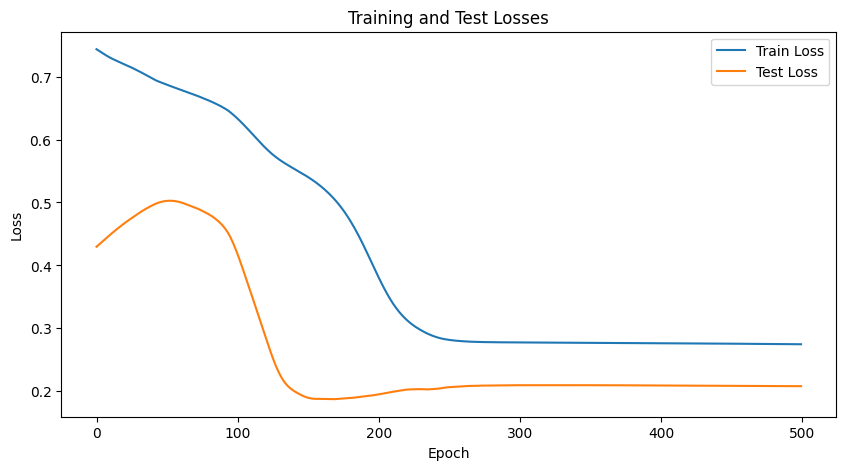
\includegraphics[width=1\linewidth]{img/C_L}
\caption{Classification loss}
\label{fig:cl}
\end{figure}

\begin{figure}[H]
\centering
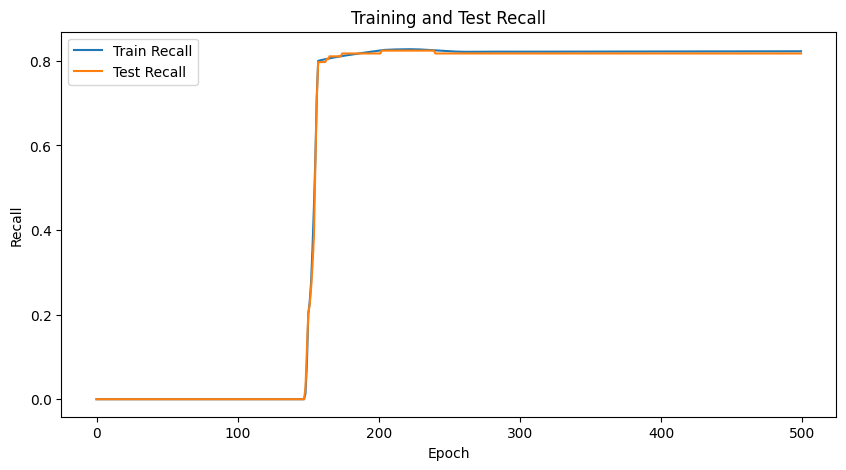
\includegraphics[width=1\linewidth]{img/C_R}
\caption{Classification Recall}
\label{fig:cr}
\end{figure}

\begin{figure}[H]
\centering
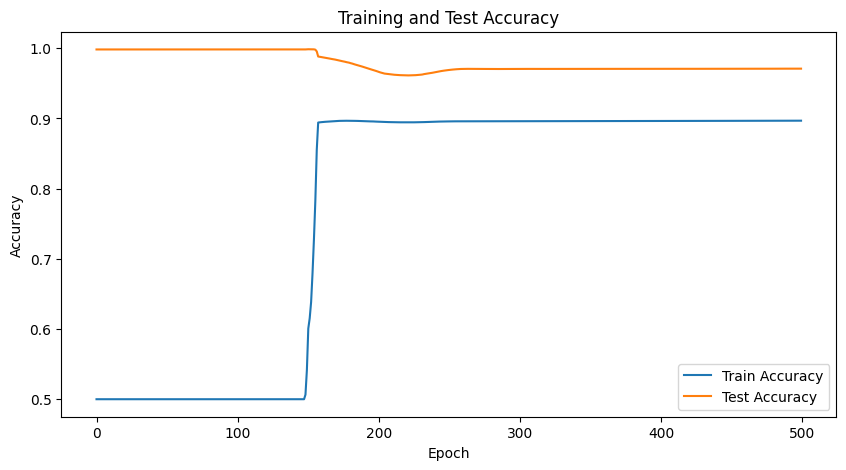
\includegraphics[width=1\linewidth]{img/C_A}
\caption{Classification Accuracy}
\label{fig:ca}
\end{figure}

\subsection{بخش چهارم}
متریک‌های مورد نظر به شرح زیر است.
\begin{LTR}
\begin{verbatim}
Classification Report:
               precision    recall  f1-score   support

           0       1.00      0.97      0.99     85295
           1       0.05      0.80      0.09       148

    accuracy                           0.97     85443
   macro avg       0.52      0.88      0.54     85443
weighted avg       1.00      0.97      0.98     85443
\end{verbatim}
\end{LTR}
و ماتریس درهم‌ریختگی در 
\autoref{fig:ccm}
 نشان داده شده است. با توجه به گزارشات و ماتریس درهم‌ریختگی عملکرد مدل در پیدا کردن نمونه‌های تقلبی با توجه به متریک Recall قبول است اما اکر مترین Precision و F1-Score را بررسی کنیم در مورد کلاس 1 نتایج خیلی بد است که این مسئله نشان می‌دهد مدل تعداد زیادی از نمونه‌های نرمال را به عنوان تقلب تشخیص داده است اما به لحاظ عملی شاید این مسئله مشکلی اساسی نباشید زیرا عدم تشخیص یک مورد تقلب می‌تواند تبعات سنگینی داشته باشد اما تشخیص یک مورد نرمال به عنوان تقلب نهایتا باعث به تاخیر افتادن گردش مالی خواهد شد که این مسئله خطر کمتری دارد. 
\begin{figure}[H]
\centering
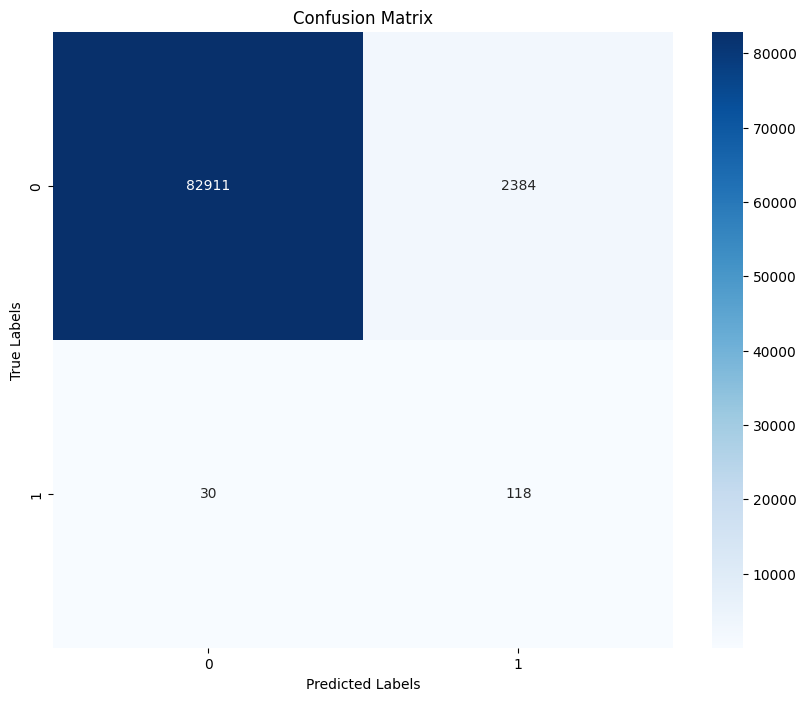
\includegraphics[width=0.7\linewidth]{img/C_cm}
\caption{Confusion matrix}
\label{fig:ccm}
\end{figure}

به منظور بررسی عملکرد متریک Accuracy در مسائلی که imbalance هستند باید به ‎ \autoref{fig:ccm}‎رجوع کرد که درایه‌های آن در فرمول ‎\autoref{facc}‎ قرار می‌گیرد. با توجه به فرمول Accuracy، مقادیر روی قطر اصلی ماتریس درهم‌ریختگی در صورت و مخرج قرار دارند و باقی مقادیر تنها در مخرج قرار دارند اما با توجه با این فرمول و اعداد موجوذ ذر ماتریس، مشخصا مقدار TN به قدری زیاد است که تمام خانه‌های دیگر ماتریس در مقابل آن قابل صرف‌نظر می‌باشد که در نتیجه آن اگر تمام نمونه‌های تقلب هم به عنوان نرمال شناسایی شود، نتیجه محسوسی در این متریک مشاهده نخواهد شد، بنابراین در این مدل مسائل Accuracy اصلا متریک خوبی نیست و اگر مدل تمام نمونه‌ها را نرمال تشخیص دهد باز عدد خیلی بالایی را نتیجه می‌دهد.

باتوجه به تحلیل مقاله، متریک Recall در کنار Accuracy می‌تواند نشان‌دهنده عملکرد مدل شود زیرا Recall تنها روی  سطر دوم ‎\autoref{fig:ccm} اجرا می‌شود و به خانه اول این ماتریس کاری ندارد و در نتیجه آن اگر مدل تمام نمونه‌ها را نرمال تشخیص دهد میزان این متریک 0 می‌شود. در کنار این متریک Precision که روی ستون دوم ماتریس عمل می‌کند و f1-score که توازنی بین Recall و Precision برقرار می‌کند نیز کمک کننده می‌باشد.

\subsection{بخش پنجم}
با استفاده از تابع زیر مقادیر به ازای thresholdهای متفاوت حساب شده است.

\begin{LTR}
	\begin{lstlisting}[language=Python, caption=Thresholding]


def calculate_metrics(outputs, labels, thresholds):
    recalls = []
    accuracies = []

    for threshold in thresholds:
        predictions = (outputs > threshold).astype(int)
        recall = recall_score(labels, predictions)
        accuracy = accuracy_score(labels, predictions)
        recalls.append(recall)
        accuracies.append(accuracy)

    return recalls, accuracies
   	\end{lstlisting}
   \end{LTR} 
که نتیجه اجرای کد فوق در ‎\autoref{fig:crat}‎ قابل مشاهده می‌باشد.
\begin{figure}[H]
\centering
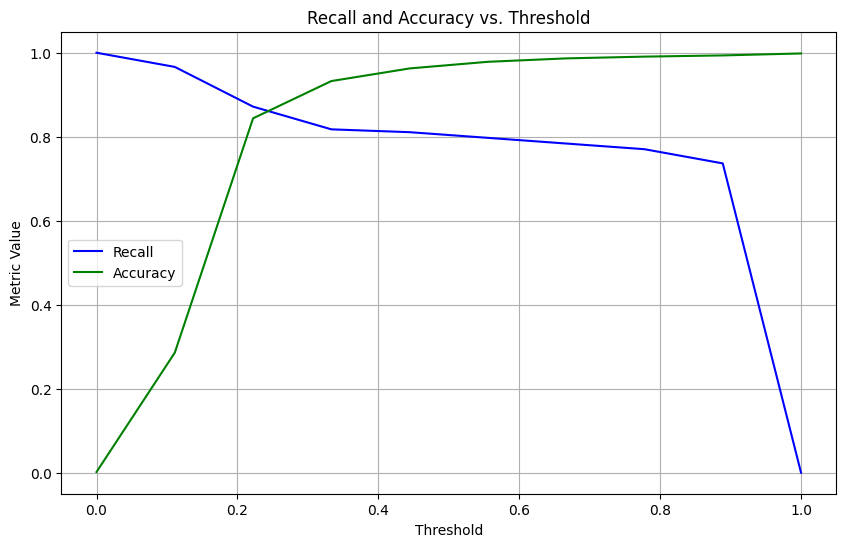
\includegraphics[width=1\linewidth]{img/C_RA_T}
\caption{Threshold effect on accuracy and recall}
\label{fig:crat}
\end{figure}


\subsection{بخش ششم}


تمام قسمت‌های قبلی را روی دیتاست موجود اجرا می‌کنیم با این تفاوت که بلاک Over-sampling اجرا نخواهد شد. نمودارها و نتایج این آزمایش در ادامه گزارش شده است. 

\begin{figure}[H]
\centering
\includegraphics[width=1\linewidth]{"img/DAE loss_2"}
\caption{Loss value of train and test set on denoising auto-encoder}
\label{fig:dae-loss2}
\end{figure}


\begin{figure}[H]
\centering
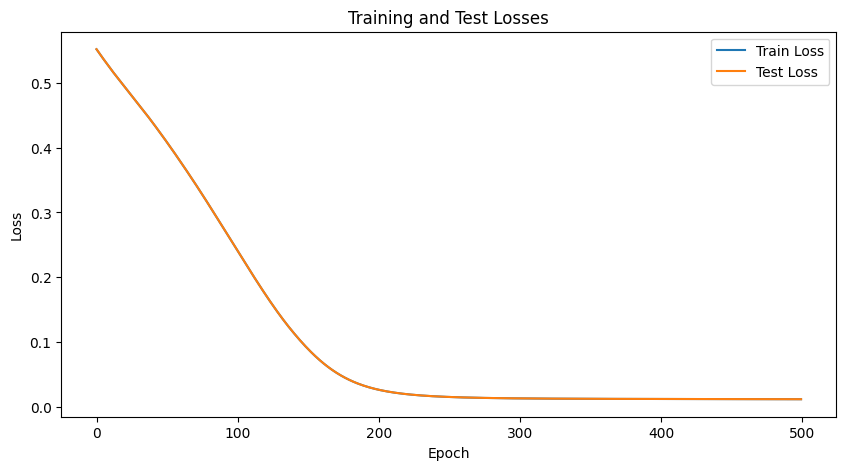
\includegraphics[width=1\linewidth]{img/C_L_2}
\caption{Loss value of training}
\label{fig:cl2}
\end{figure}

\begin{figure}[H]
\centering
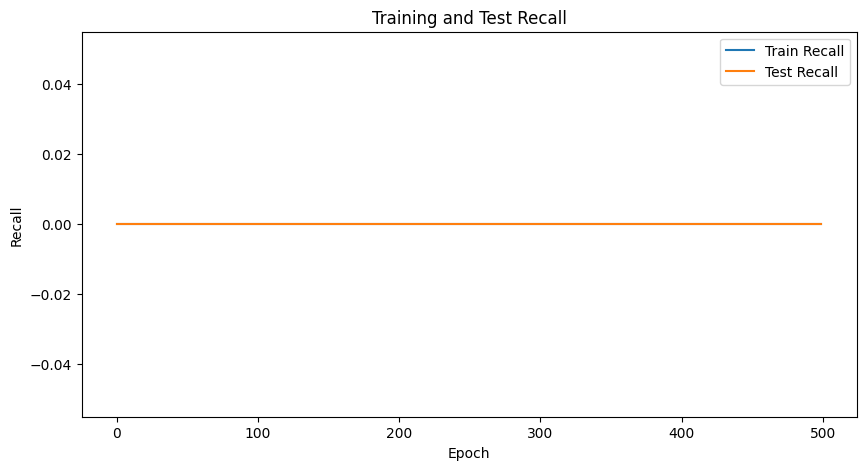
\includegraphics[width=1\linewidth]{img/C_R_2}
\caption{Recall of training}
\label{fig:cr2}
\end{figure}

\begin{figure}[H]
\centering
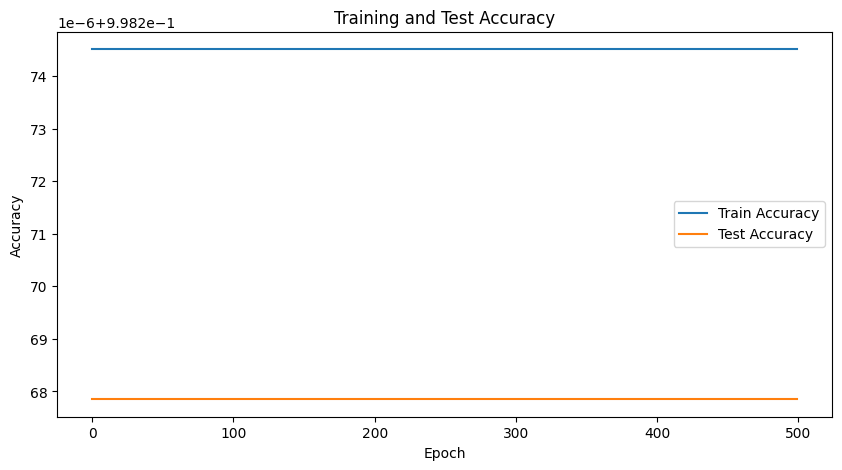
\includegraphics[width=1.0\linewidth]{img/C_A_2}
\caption{Accuracy of training}
\label{fig:ca2}
\end{figure}


\begin{LTR}

\begin{verbatim}
               precision    recall  f1-score   support

           0       1.00      1.00      1.00     85295
           1       0.00      0.00      0.00       148

    accuracy                           1.00     85443
   macro avg       0.50      0.50      0.50     85443
weighted avg       1.00      1.00      1.00     85443
\end{verbatim}
\end{LTR}

\begin{figure}[H]
\centering
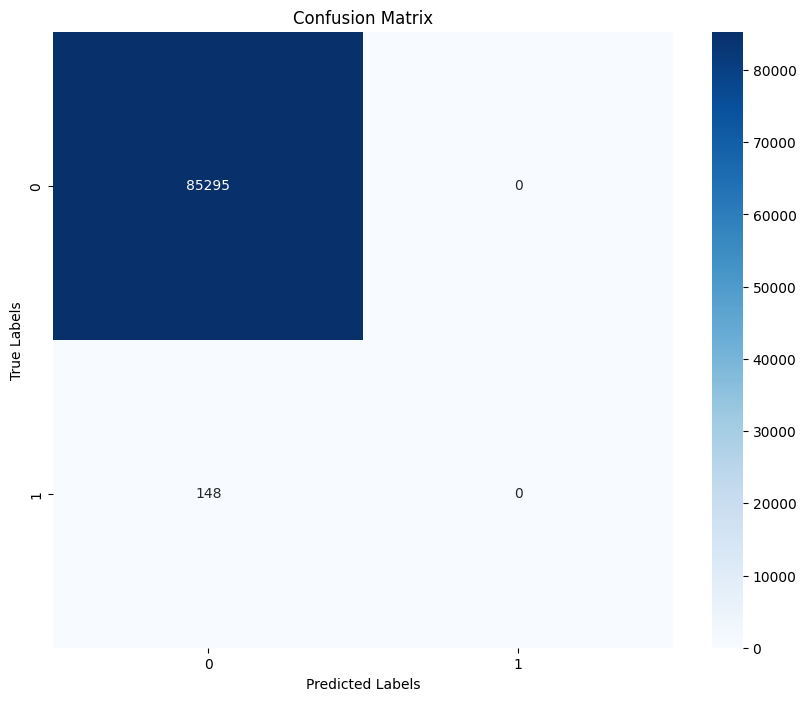
\includegraphics[width=1.0\linewidth]{img/C_cm_2}
\caption{Confusion matrix}
\label{fig:ccm2}
\end{figure}


\begin{figure}[H]
\centering
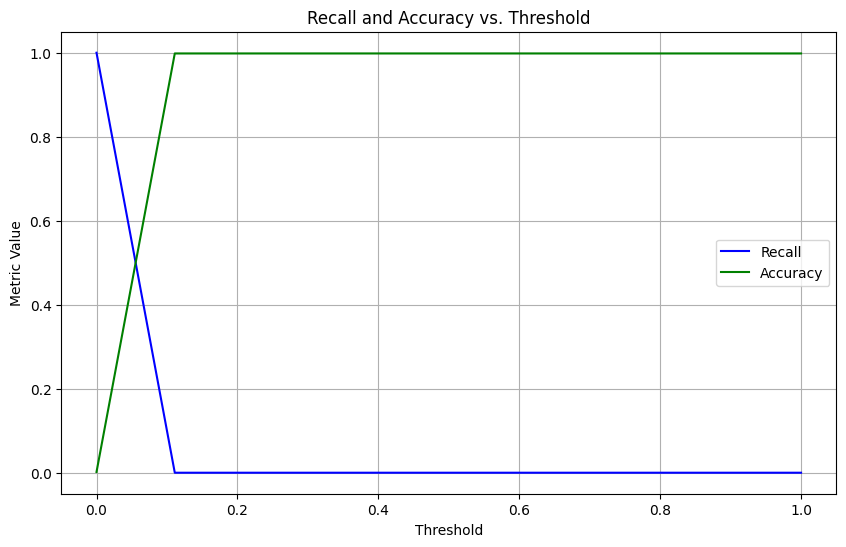
\includegraphics[width=1.0\linewidth]{img/C_RA_T_2}
\caption{Threshold effect on recall and accuracy}
\label{fig:crat2}
\end{figure}



همانطور که انتظار می‌رفت نتایج بسیار افت کرده است و اما متریک Accuracy برابر 1 شده است. اگر به ‎\autoref{fig:ccm2}‎ توجه کنیم، مشخص است که مدل تمام نمونه‌ها را به عنوان تقلب در نظر می‌گیرد که نتیجه آن این است که Recall برابر 0 خواهد شد اما accuracy به مقدار 1 بسیار نزدیک می‌شود. 





\bibliographystyle{plain}
\bibliography{references}
\end{document}

